\section{Auswertung}
\label{sec:Auswertung}

\subsection{Dampfdruck und mittlere freie Weglänge}

Zunächst wird mithilfe von \autoref{eqn:Dampfdruck} und \autoref{eqn:w} der Dampfdruck $p_{\mathrm{sät}}$ und die mittlere
freie Weglänge $\bar{w}$ in Abhängigkeit der Temperatur $T$ bestimmt und anschließend mit dem
Abstand $a$ der Kathode und der Beschleunigungselektrode verglichen, welcher etwa 1 $\si{\centi\meter}$
beträgt.\\

\begin{table}[!h]
  \begin{center}
    \begin{tabular}{|c|c|c|c|c|}
      \hline
      $T / \si{\celsius}$ & $T / \si{\kelvin}$ & $p_{\mathrm{sät}} / \si{\milli\bar}$ & $\bar{w} / \si{\centi\meter}$ & $\frac{a}{\bar{w}}$\\
      \hline
      \hline
      27  & 300,15 & 0,0061  & 0.46891 & 2,13\\
      160 & 433,15 & 7,0177  & 0.00041 & 2419,9\\
      175 & 448,15 & 11,939  & 0.00024 & 4116,72\\
      185 & 458,15 & 16,688  & 0.00017 & 5754,3\\
      \hline
    \end{tabular}
    \caption{Dampfdruck $p_\mathrm{sät}$ und mittlere freie Weglänge $\bar{w}$ in Abhängigkeit von der Temperatur $T$.}
    \label{tab:weg}
  \end{center}
\end{table}

Damit eine ausreichende Stoßwahrscheinlichkeit gegeben ist, muss $\bar{w}$ etwa um den Faktor
1000 bis 4000 größer sein als der Abstand $a$. Das ist bei allen gemessenen Temperaturen außer
den $27 \, \, \si{\celsius}$ gegeben. Hier ist das Verhältnis zu gering, als dass man eine aussagekräftige
Frank-Hertz-Kurve aufnehmen könnte.\\

\subsection{Differentielle Energieverteilung der Elektronen}

Mithilfe eines X-Y-Schreibers wurden jeweils für $27 \, \, \si{\celsius}$ und $160 \, \, \si{\celsius}$
der Auffängerstrom $I_{\mathrm{A}}$ in Abhängigkeit der Bremsspannung $U_{\mathrm{A}}$ bei einer konstanten Beschleunigungsspannung
von $U_{\mathrm{B}} = + 11 \si{\volt}$ aufgenommen.\\

\subsubsection{Messung bei 27 Grad Celsius}

Die bei $27 \, \, \si{\celsius}$ abgelesenen Werte sind in \autoref{tab:27C} zu finden, das Originalbild
des X-Y-Schreibers ist in \autoref{Abb:a} dargestellt.

\begin{figure}
  \centering
  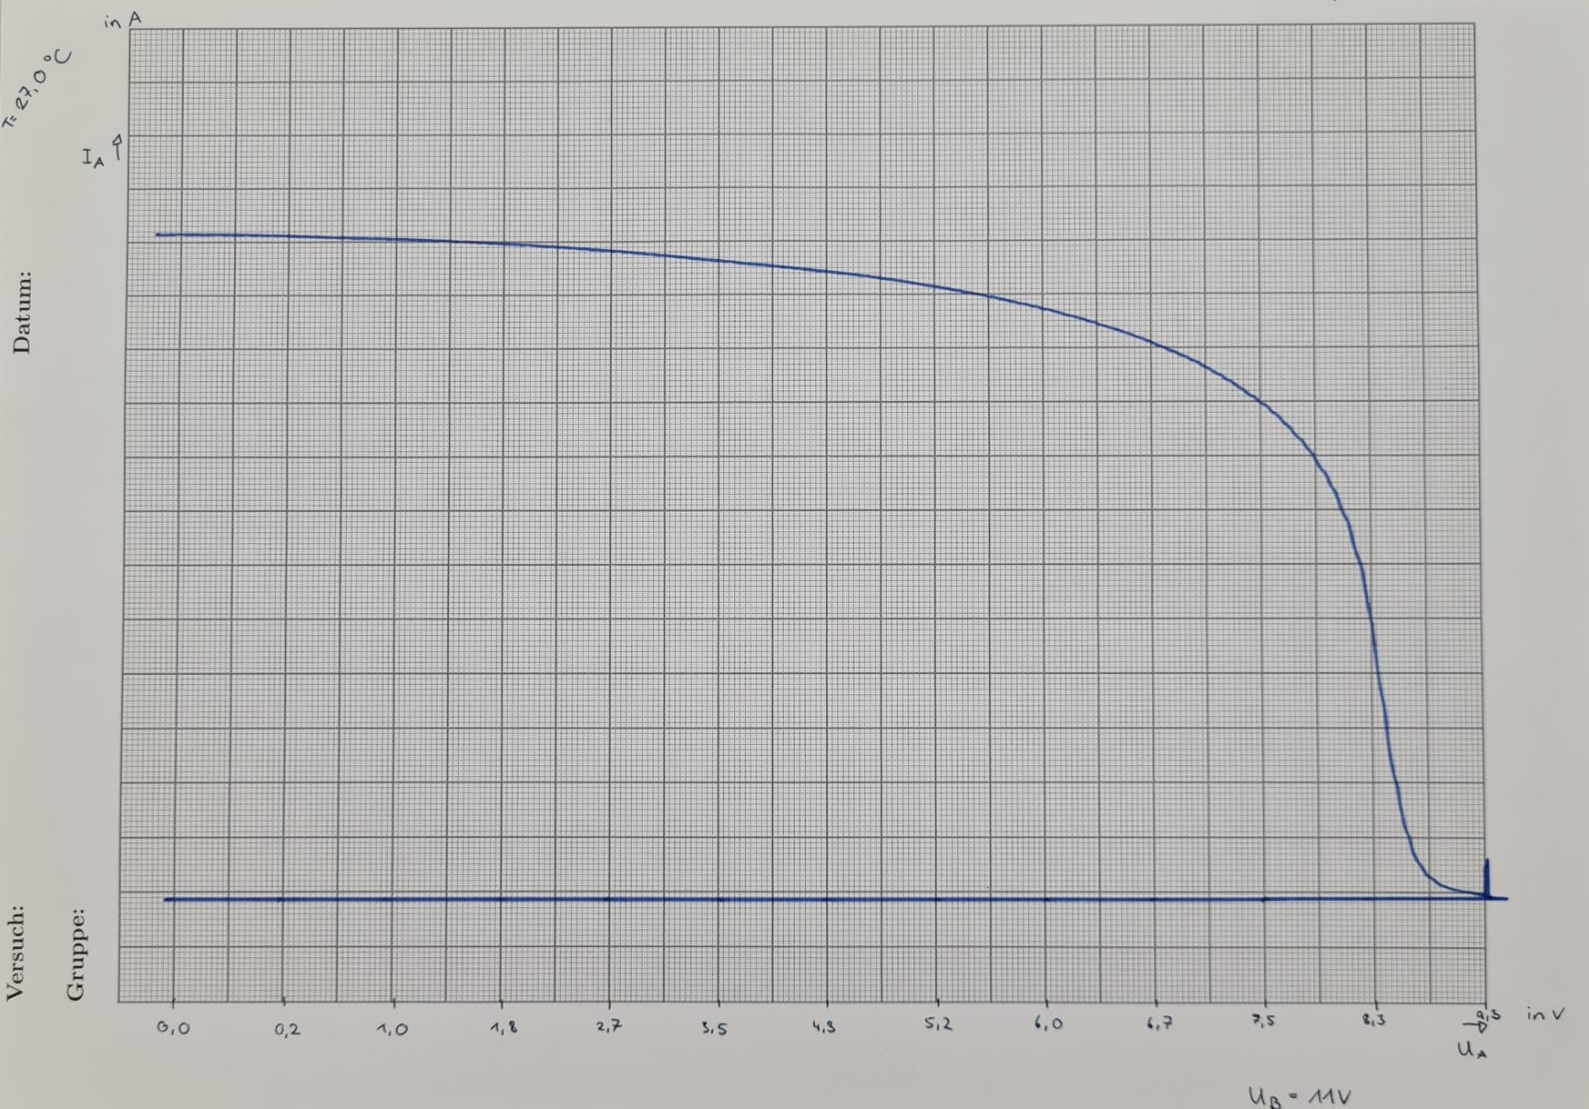
\includegraphics[height=8cm]{Messwerte/a.jpg}
  \caption{Auffängerstrom in Abhängigkeit der Bremsspannung bei $T=27\,\si{\celsius}$.}
  \label{Abb:a}
\end{figure}


\begin{table}[!h]
  \begin{center}
    \begin{tabular}{|c|c|c||c|c|c|}
      \hline
      $U_{\mathrm{A}} / \si{\volt}$ & $\Delta U_{\mathrm{A}} / \si{\volt}$ & $\Delta I_{\mathrm{A}} / \si{\ampere}$ & $U_{\mathrm{A}} / \si{\volt}$ & $\Delta U_{\mathrm{A}} / \si{\volt}$ & $\Delta I_{\mathrm{A}} / \si{\ampere}$\\
      \hline
      0,2 & 0,2 & 0,1 & 5,2 & 0,9 & 3  \\
      1,0 & 0,8 & 1   & 6,0 & 0,8 & 5  \\
      1,8 & 0,8 & 1   & 6,7 & 0,7 & 6 \\
      2,7 & 0,9 & 2   & 7,5 & 0,8 & 11 \\
      3,5 & 0,8 & 2   & 8,3 & 0,8 & 40 \\
      4,3 & 0,8 & 3   & 8,8 & 0,5 & 46 \\
      4,3 & 0,8 & 3   & 9,3 & 0,5 & 5 \\
      \hline
    \end{tabular}
    \caption{Lokale Auffängerstromänderung $\Delta I_{\mathrm{A}}$ in den Intervallen $\Delta U_{\mathrm{A}}$  bei $27 \, \si{\celsius}$}
    \label{tab:27C}
  \end{center}
\end{table}

Um die differentielle Energieverteilung der Elektronen zu bestimmen, werden in der aufgenommenen 
Graphik jeweils für bestimmte Intervalle $\Delta U_{\mathrm{A}}$ und $\Delta I_{\mathrm{A}}$ aufgenommen, also jeweils
kleine einzelne Steigungsdreiecke. Die Größe von den $\Delta I_{\mathrm{A}}$'s 
sind anhand der einzelnen Kästchen des Millimeterpapiers frei bestimmt. 1 LE = 1 Kästchen.\\
Die gewählten Intervalle für $\Delta U_{\mathrm{A}}$ sind in \autoref{Abb:a} und in \autoref{tab:27C} abzulesen.\\
Die Werte für $\Delta I_{\mathrm{A}}$ werden nun gegen $\Delta U_{\mathrm{A}}$ geplottet. Der in \autoref{fig:27GradDiff} entstehende Verlauf
beschreibt die differentielle Energieverteilung.\\

\begin{figure}[H]
  \centering
  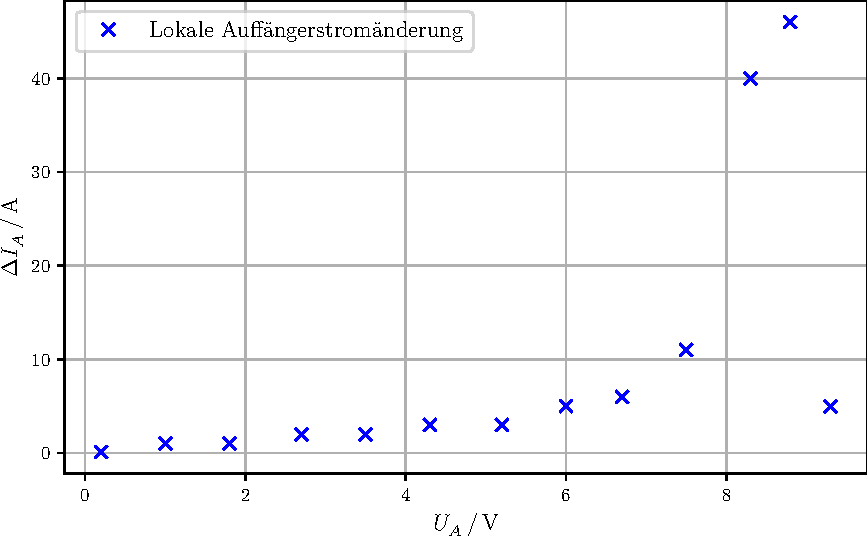
\includegraphics[height=8cm]{build/27Grad.pdf}
  \caption{Differentielle Energieverteilung der Elektronen bei $T=27\,\si{\celsius}$.}
  \label{fig:27GradDiff}
\end{figure}

Es lässt sich erkennen, dass die lokale Änderungsrate des Auffängerstroms
bei $U_{\mathrm{A}} = 8,8 \si{\volt}$ ein Maximum annimmt und danach wieder sinkt. Das heißt,
dass die meisten Elektronen eine Energie von circa $E_{\mathrm{Z}} = e_0 \cdot U_A = (14,0976 \cdot 10^{-19}) \, \si{\joule}$
haben.\\
Das Kotaktpotential ergibt sich aus der Differenz der Beschleunigungsspannung $U_{\mathrm{B}}$ und der Spannung
des Maximums der Kurve und wird mit der Gleichung
\begin{equation}
  K = U_{\mathrm{B}} - U_{\mathrm{A,max}} = 2,2 \si{\volt}
\end{equation}
berechnet.\\

\subsubsection{Messung bei 160 Grad Celsius}

Die Auswertung für $160 \, \si{\celsius}$ erfolgt analog zu der für $27 \, \si{\celsius}$.
Die jeweiligen Messwerte und das Originalbild lassen sich in \autoref{tab:160C} und 
\autoref{Abb:160C} finden.

\begin{figure}
  \centering
  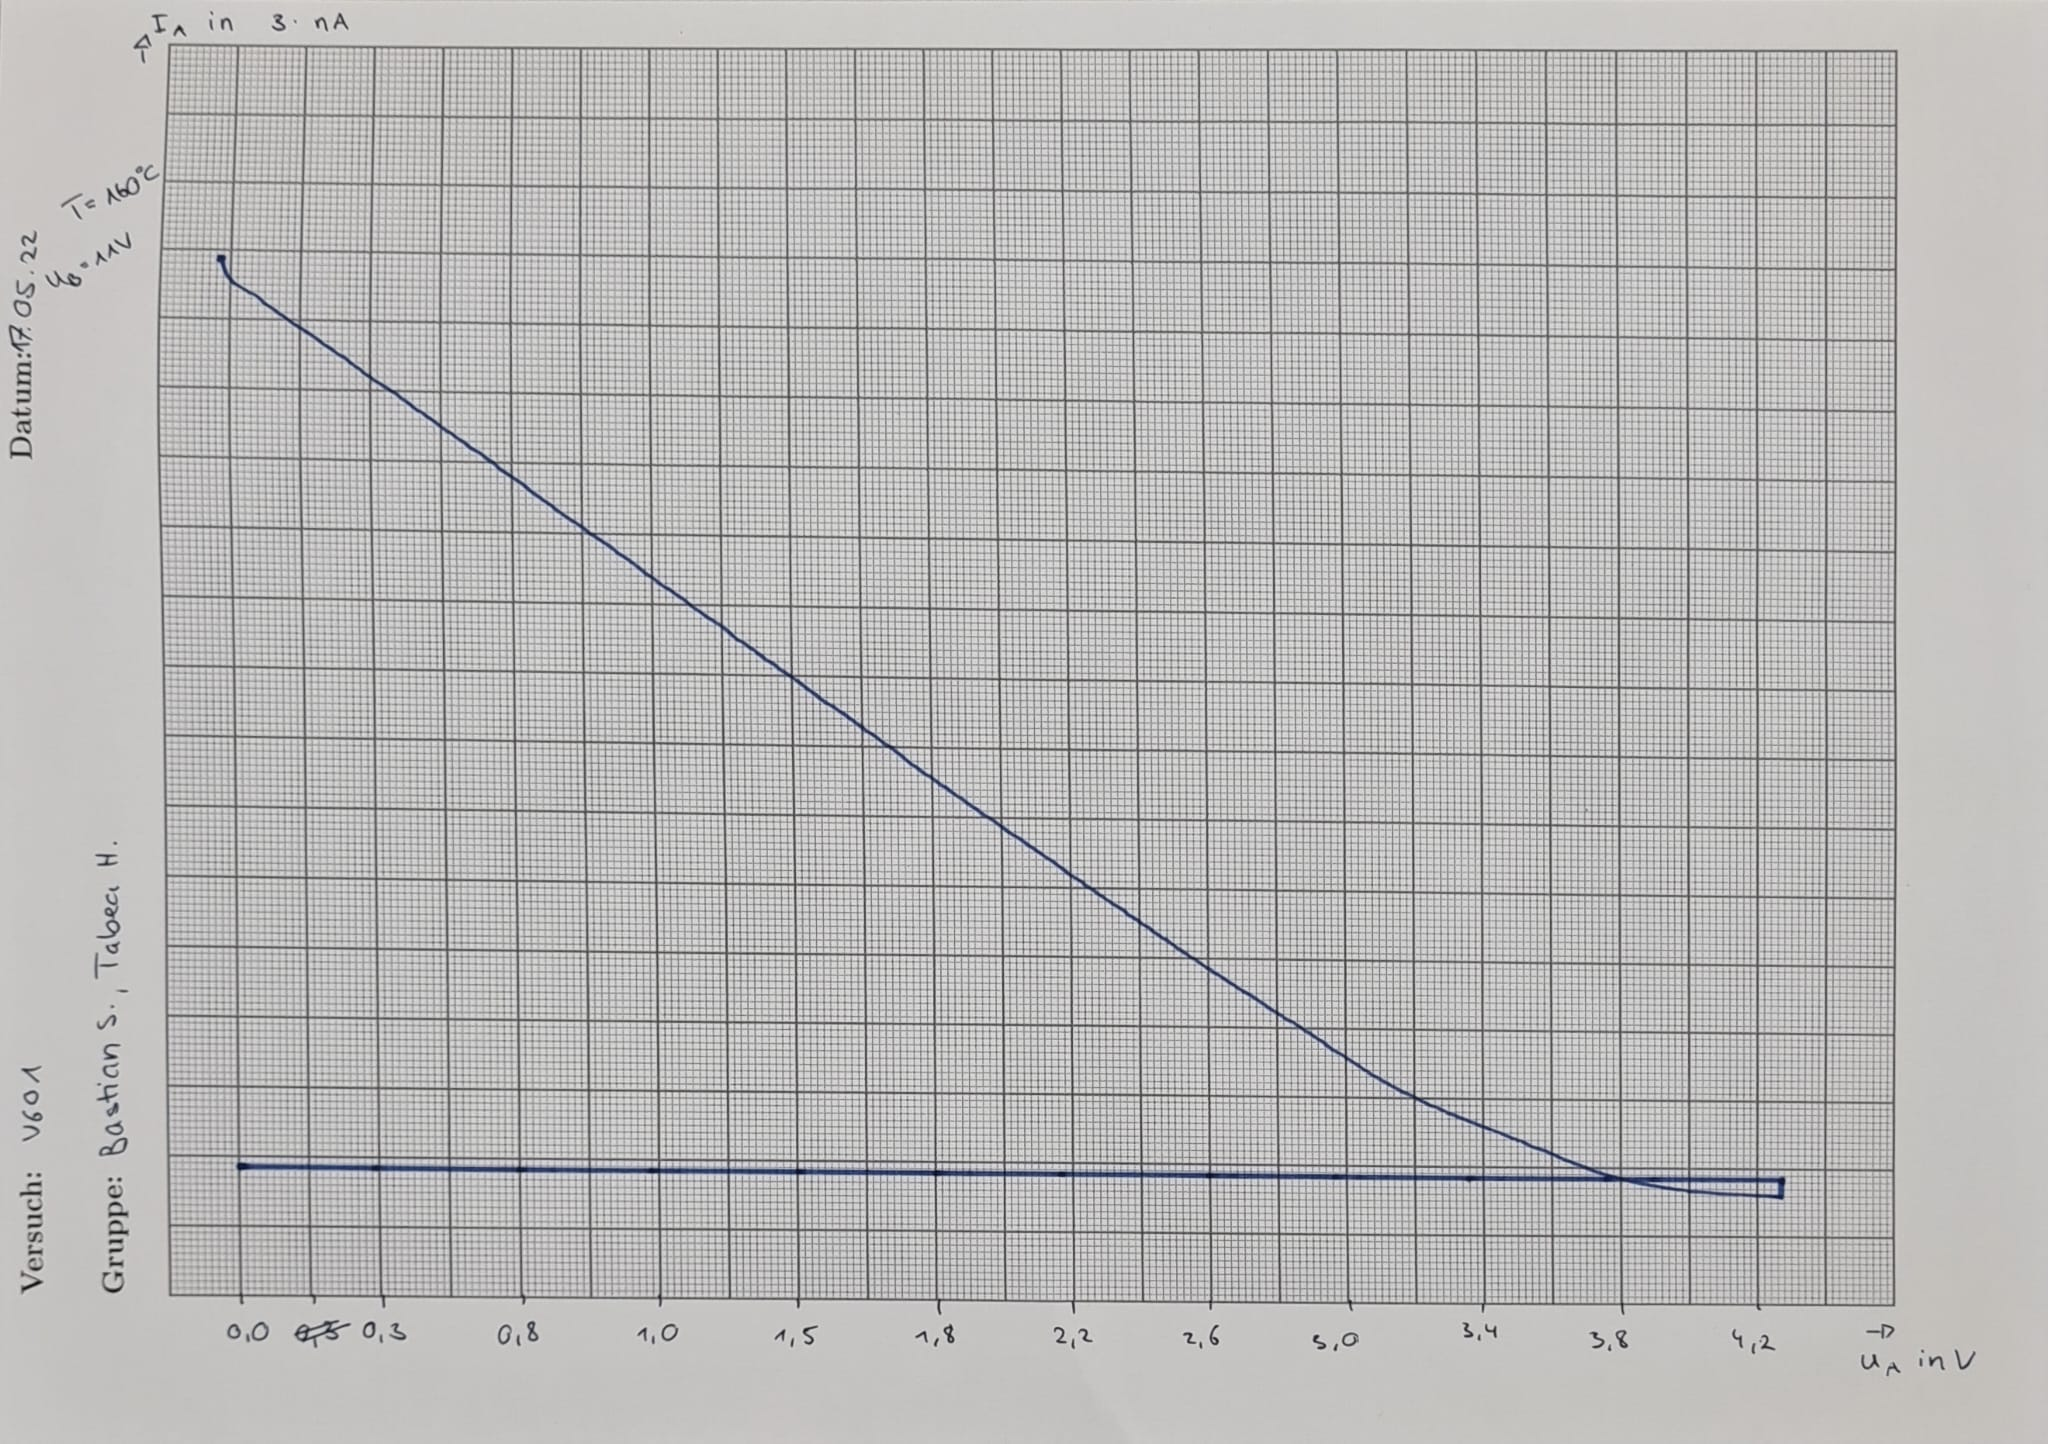
\includegraphics[height=8cm]{Messwerte/b.jpg}
  \caption{Auffängerstrom in Abhängigkeit der Bremsspannung bei $T=160\,\si{\celsius}$.}
  \label{Abb:160C}
\end{figure}

\begin{table}[!h]
  \begin{center}
    \begin{tabular}{|c|c|c||c|c|c|}
      \hline
      $U_{\mathrm{A}} / \si{\volt}$ & $\Delta U_{\mathrm{A}} / \si{\volt}$ & $\Delta I_{\mathrm{A}} / \si{\ampere}$ & $U_{\mathrm{A}} / \si{\volt}$ & $\Delta U_{\mathrm{A}} / \si{\volt}$ & $\Delta I_{\mathrm{A}} / \si{\ampere}$\\
      \hline
      0,3 & 0,3 & 14 & 2,6 & 0,4 & 13  \\
      0,8 & 0,5 & 14 & 3,0 & 0,4 & 12  \\
      1,0 & 0,2 & 14 & 3,4 & 0,4 & 10  \\
      1,5 & 0,5 & 14 & 3,8 & 0,4 & 8  \\
      1,8 & 0,3 & 14 & 4,2 & 0,4 & 2 \\
      2,2 & 0,4 & 14 & & & \\
      \hline
    \end{tabular}
    \caption{Lokale Auffängerstromänderung $\Delta I_{\mathrm{A}}$ in den Intervallen $\Delta U_{\mathrm{A}}$ bei $160 \, \si{\celsius}$}
    \label{tab:160C}
  \end{center}
\end{table}

Die Werte werden erneut gegeneinander geplottet. Die entstandene Kurve ist in \autoref{fig:160GradDiff}
zu sehen.\\

\begin{figure}[H]
  \centering
  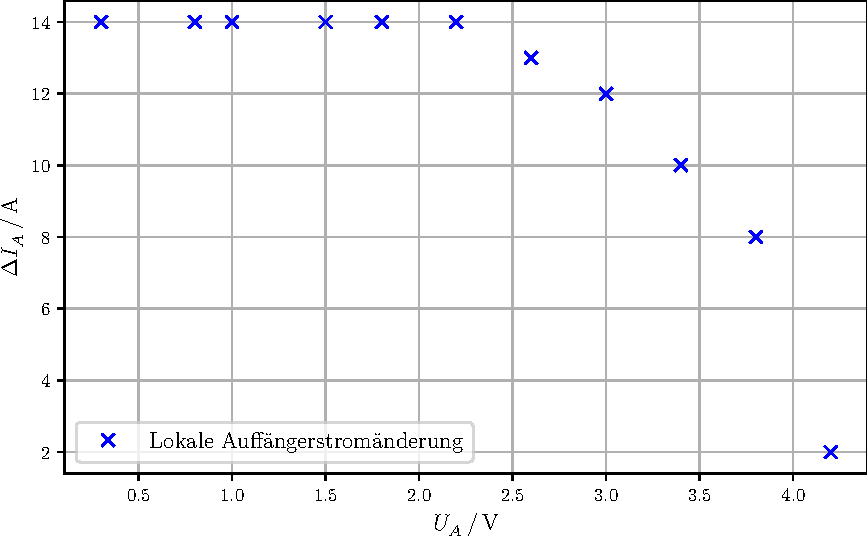
\includegraphics[height=8cm]{build/160Grad.pdf}
  \caption{Differentielle Energieverteilung der Elektronen bei $T=160\,\si{\celsius}$.}
  \label{fig:160GradDiff}
\end{figure}

Es ist zu erkennen, dass der Auffängerstrom konstant abfällt bis dieser einen Wert Null erreicht.\\
Aufgrund der wesentlich höheren Temperatur finden mehr elastische Stöße zwischen den Elektronen
und dem Quecksilber-Dampf, bestehend aus Hg-Atomen statt.\\
Durch die elastischen Stöße werden die Elektronen gestreut und haben dadurch einen geringeren
Anteil an kinetischer Energie in Feldrichtung.\\
Der Grund dafür, dass die Verteilung ab ca 4,8 V Null bleibt, ist dass die Anregungsenergie des
Quecksilberatoms nach dem berechneten Wert im nächsten Aufgabenteil ca. 4,9 eV beträgt. Wenn nun Elektronen mit dieser oder größerer
Energie auf ein Hg-Atom treffen, wird diese Anregungsenergie an die äußeren Elektronen des Atoms
übertragen.\\
Leider lässt sich der Bereich nach 4 V nicht mehr in der Abbildung beobachten. Es ist jedoch
stark anzunehmen, dass aufgrund vorheriger Erklärung der Auffängerstrom nicht wieder ansteigt.

\subsection{Franck-Hertz-Kurven}

Zur Bestimmung der Anregungsenergie des Hg-Atoms werden jeweils eine Franck-Hertz-Kurve
bei $T=175 \, \si{\celsius}$ und $T=185 \, \si{\celsius}$ ausgewertet und aus diesem Wert
die Wellenlänge der beim Übergang in den Grundzustand emittierten Strahlung bestimmt.\\
Es wird die Beschleunigungsspannung $U_{\mathrm{B}}$ variiert und die Bremsspannung $U_{\mathrm{A}}$ konstant auf
1 V gehalten.

\subsubsection{Franck-Hertz-Kurve bei 175 Grad Celsius}

Es werden jeweils die Abstände der Peaks zueinander bestimmt und dann der Mittelwert
dessen Werte. Die Abstände $\Delta U_{\mathrm{B}}$ sind in \autoref{tab:UB175} aufgelistet.

\begin{table}[!h]
  \begin{center}
    \begin{tabular}{|c|c|c|}
      \hline
      $\mathrm{Nr. Peak} $ & $U_{\mathrm{A}} / \si{\volt}$ & $\Delta U_{\mathrm{A}} / \si{\volt}$ \\
      \hline
      1 & 5,7 & \\
      2 & 10,9 & 5,2 \\
      3 & 15,5 & 4,6 \\
      4 & 20   & 4,7 \\
      5 & 25,5 & 5,5 \\
      \hline
    \end{tabular}
    \caption{Abstände der Maxima des Auffängerstroms bei $175 \, \si{\celsius}$}
    \label{tab:UB175}
  \end{center}
\end{table}

Mittels der Python Uncertainties Bibliothek \cite{python} ergibt sich der Mittelwert der Abstände der Peaks, also
die Anregungsenergie zu $\bar{E_1} = (5,0 \pm 0,4) \, \si{\electronvolt}$. \\
Mit $E = h \frac{c}{\lambda}$ ergibt sich anschließend auch die Wellenlänge der beim Übergang in den
Grundzustand emittierten Strahlung mit $\lambda_1 = (248 \pm 18) \, \si{\nano\meter}$.\\
Das mittels X-Y-Schreibers aufgenommene Bild ist in \autoref{Abb:c} dargestellt.

\begin{figure}[H]
  \centering
  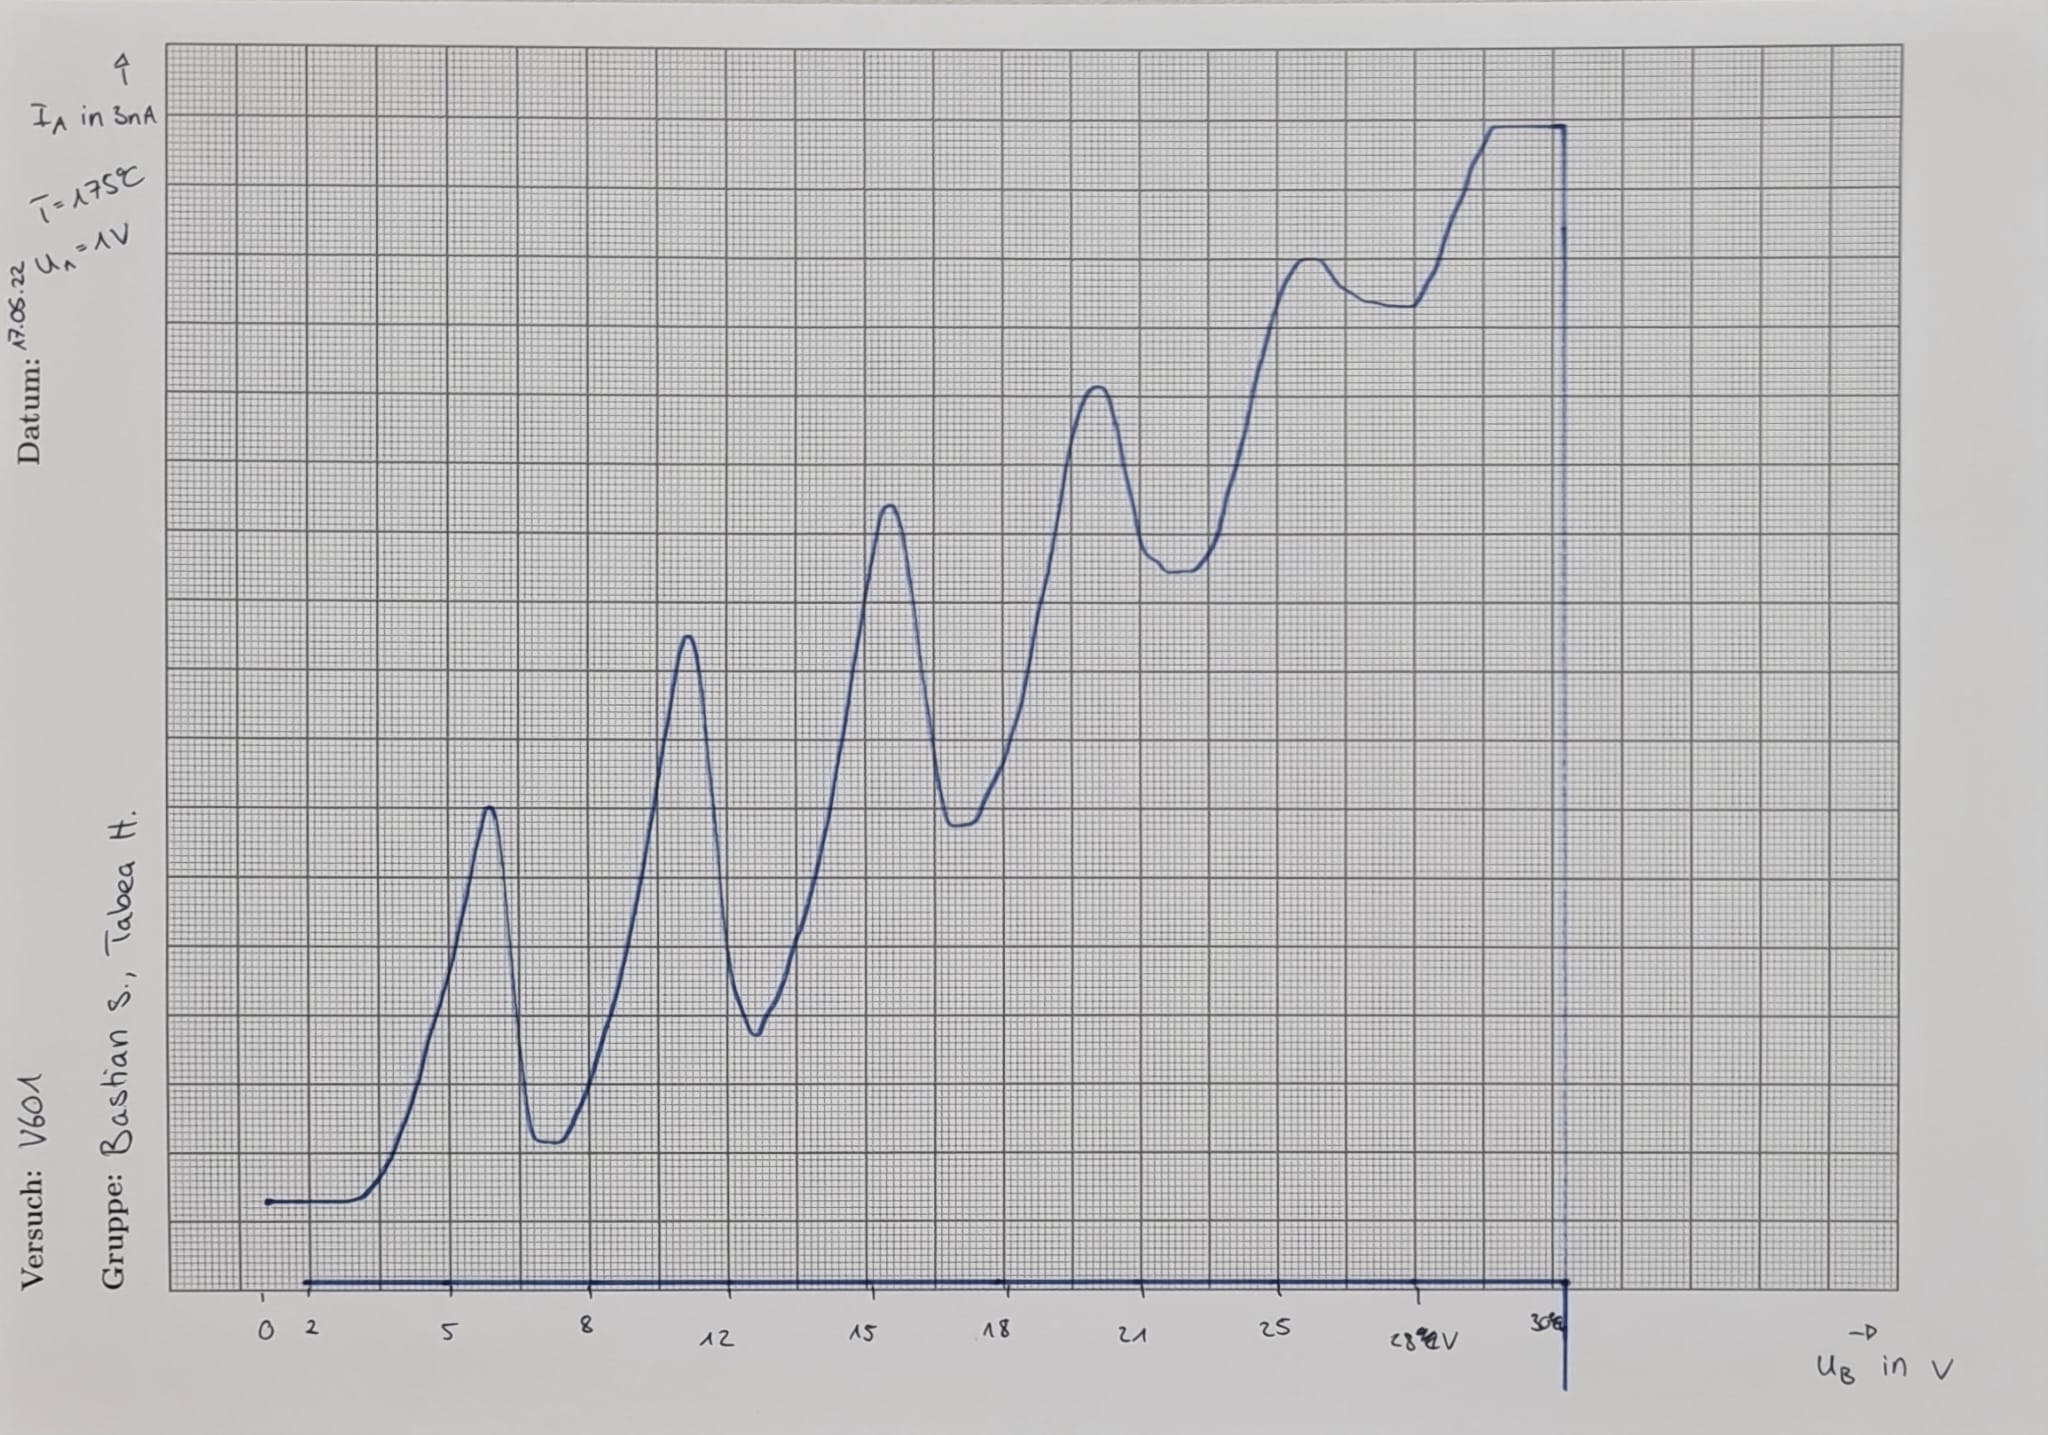
\includegraphics[height=8cm]{Messwerte/c.jpg}
  \caption{Franck-Hertz-Kurve bei $T=175\,\si{\celsius}$.}
  \label{Abb:c}
\end{figure}

\subsubsection{Franck-Hertz-Kurve bei 185 Grad Celsius}

Für die Franck-Hertz-Kurve bei $185 \, \si{\celsius}$ wird genau gleich vorgegangen.\\
Die Abstände der Peaks lassen sich in \autoref{tab:UB185} wiederfinden.

\begin{table}[!h]
  \begin{center}
    \begin{tabular}{|c|c|c|}
      \hline
      $\mathrm{Nr. Peak} $ & $U_{\mathrm{A}} / \si{\volt}$ & $\Delta U_{\mathrm{A}} / \si{\volt}$ \\
      \hline
      1 & 5,8 & \\
      2 & 10,5 & 4,7 \\
      3 & 15,2 & 4,7 \\
      4 & 20,1 & 4,9 \\
      5 & 25,1 & 5,0 \\
      6 & 29,8 & 4,7 \\
      \hline
    \end{tabular}
    \caption{Abstände der Maxima des Auffängerstroms bei $185 \, \si{\celsius}$}
    \label{tab:UB185}
  \end{center}
\end{table}

Mithilfe Python ergibt sich nun erneut die Anregungsenergie und die Wellenlänge der emittierten
Strahlung zu $\bar{E_2} = (4,8 \pm 0,13) \, \si{\electronvolt}$ und $\lambda_2 = (259 \pm 7) \, \si{\nano\meter}$.\\
Das aufgezeichnete Bild lässt sich in \autoref{Abb:d} betrachten.

\begin{figure}[H]
  \centering
  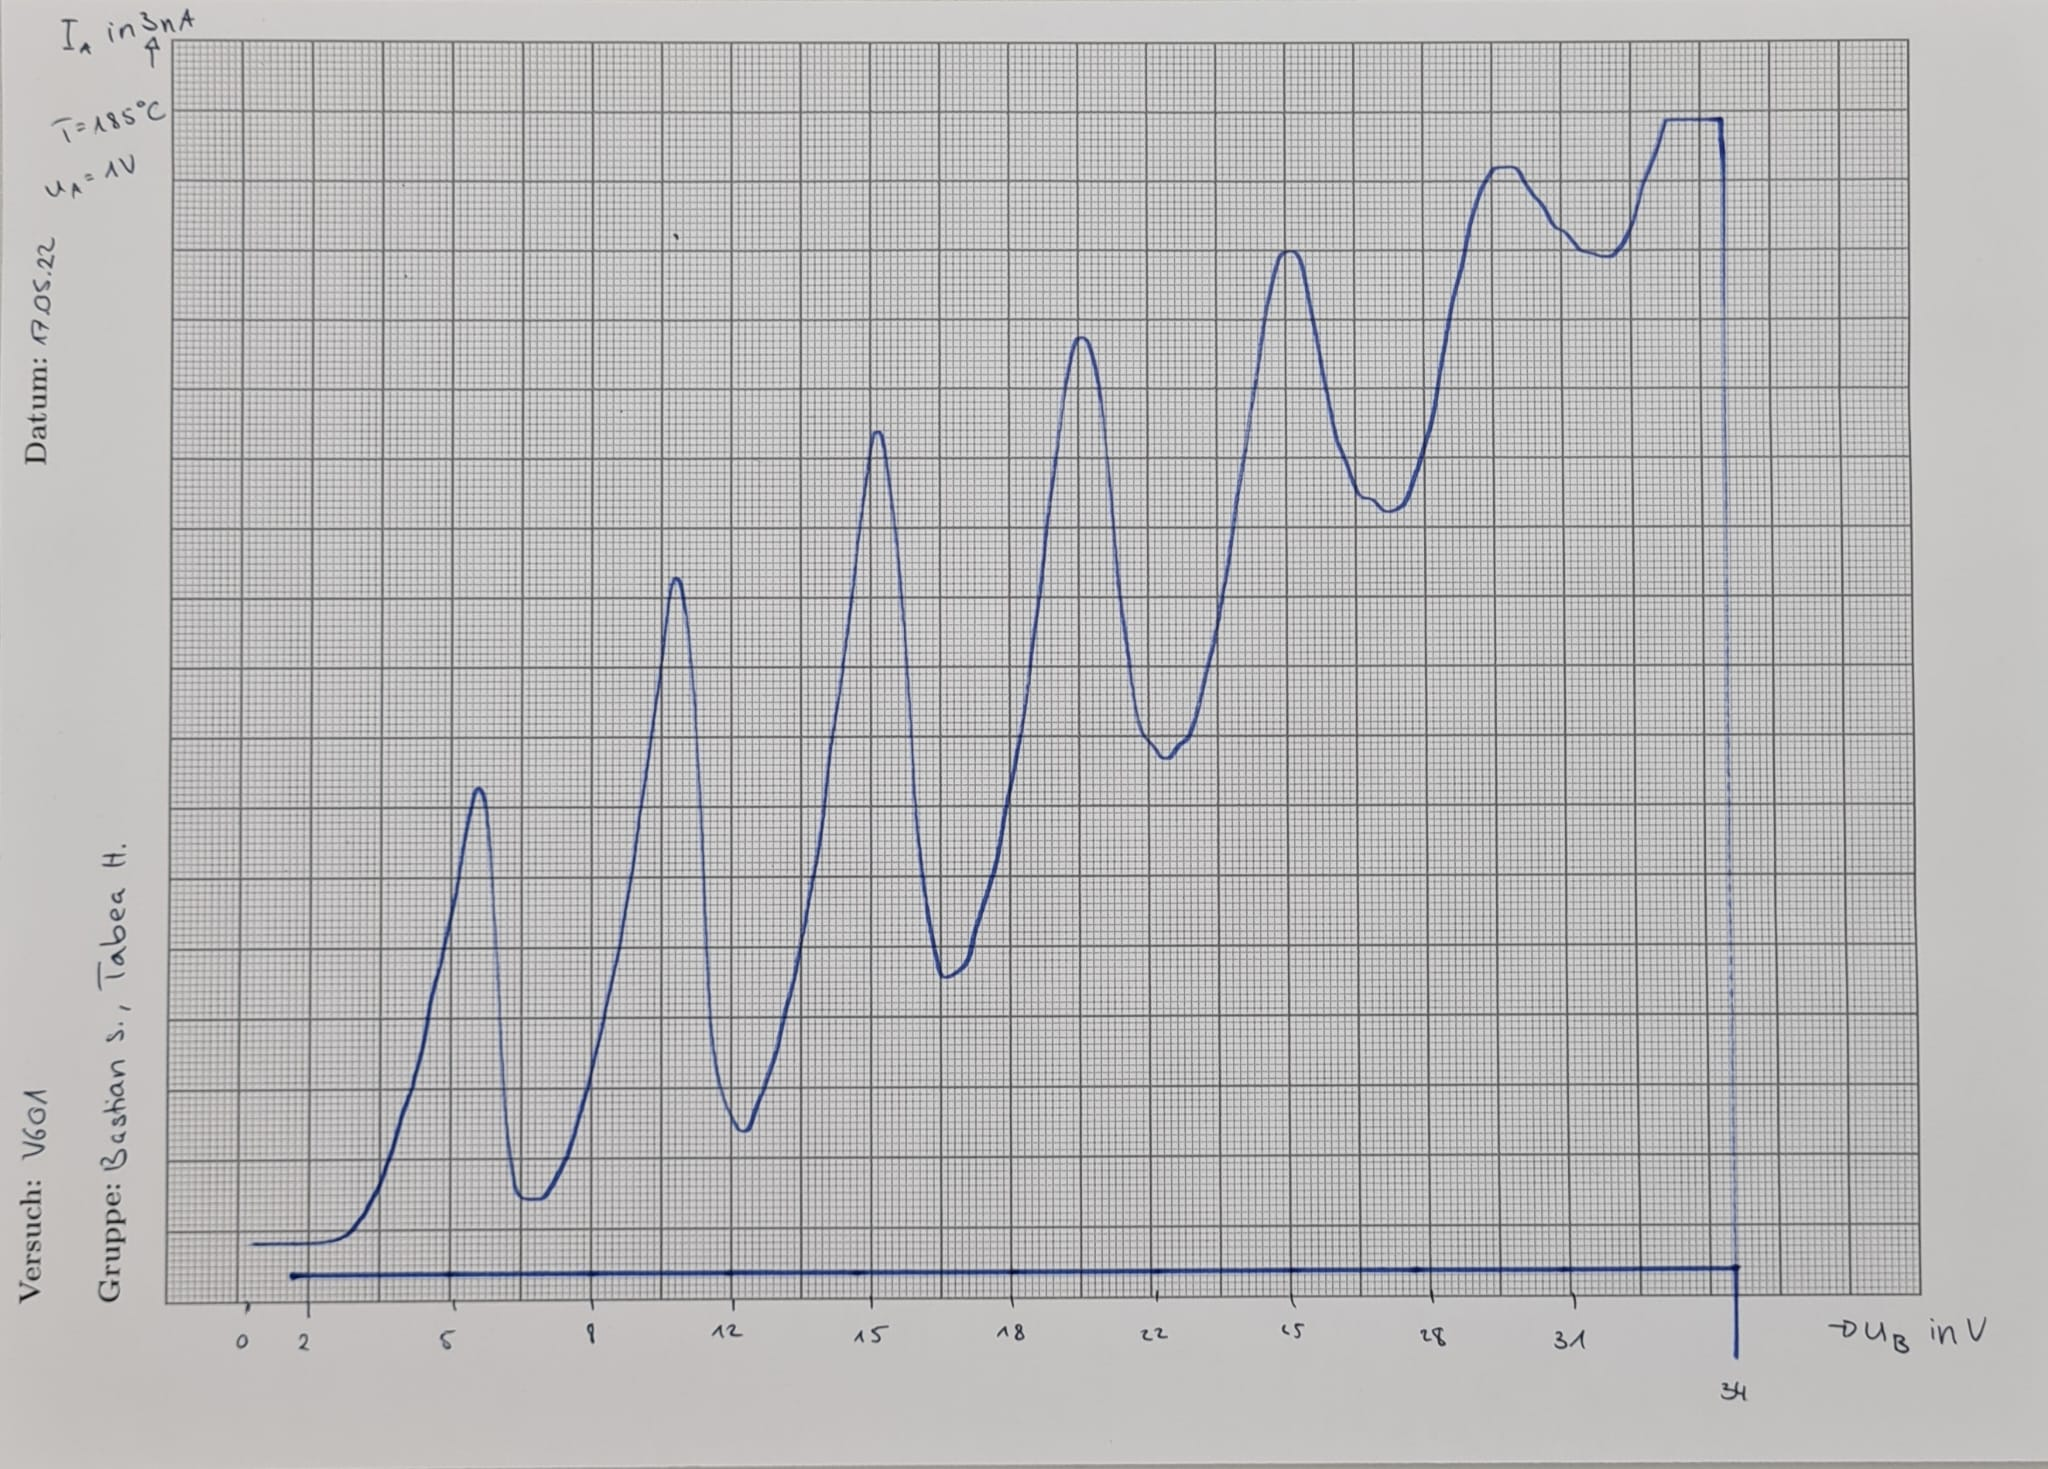
\includegraphics[height=8cm]{Messwerte/d.jpg}
  \caption{Franck-Hertz-Kurve bei $T=185\,\si{\celsius}$.}
  \label{Abb:d}
\end{figure}

Anders als im vorherigen Versuchsteil beinflussen die vielen elastischen Stöße hier nicht
die Qualität der Messergebnisse, da lediglich die Höhe der Peaks und nicht die Abhängigkeit
von $U_{\mathrm{B}}$ beeinflusst wird.  